\documentclass{tufte-handout}

\usepackage{graphicx,amsmath}

\title{Probability Distributions}
\author{}
\date{}

\begin{document}
\maketitle

\section{Binomial Distribution}
\begin{figure}
    \caption{Binomial Distribution}
    \centering
    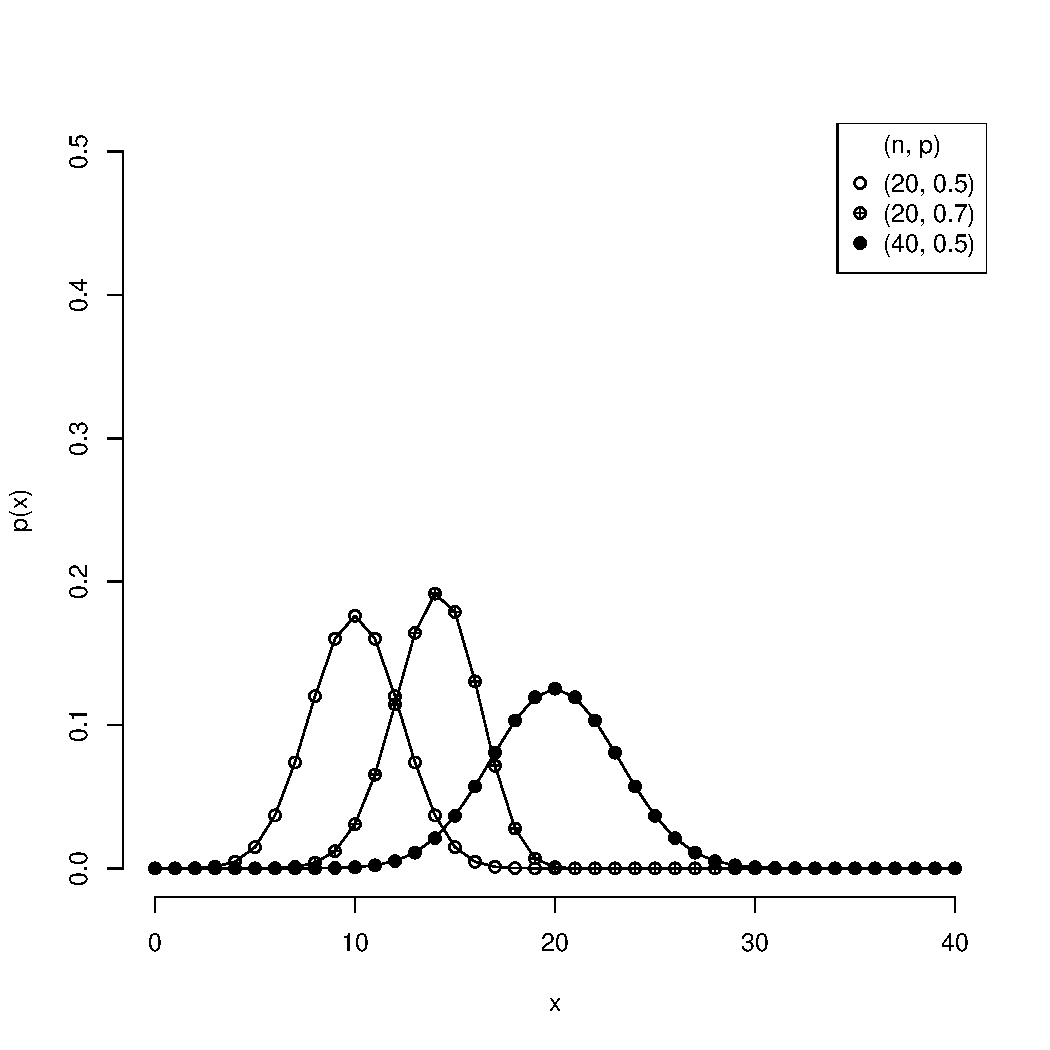
\includegraphics[width=.70\textwidth]{../distributions/binomial/binomial_bw.pdf}
\end{figure}
\marginnote[-3.0in]{
    \begin{align*}
        & X \sim \text{Binomial} (n, p) \\
        & x = 0, 1, 2, \dots, n \\
        & 0 < p < 1 \\
        & p(x) = {n \choose x} p^x (1-p)^{x-1} \\
        & \mu = E[X] = np \\
        & \sigma^2 = E[(x-\mu)^2] = np(1-p) \\
    \end{align*}
}

\section{Normal Distribution}
\begin{figure}
    \caption{Normal$(0,1)$ Distribution}
    \centering
    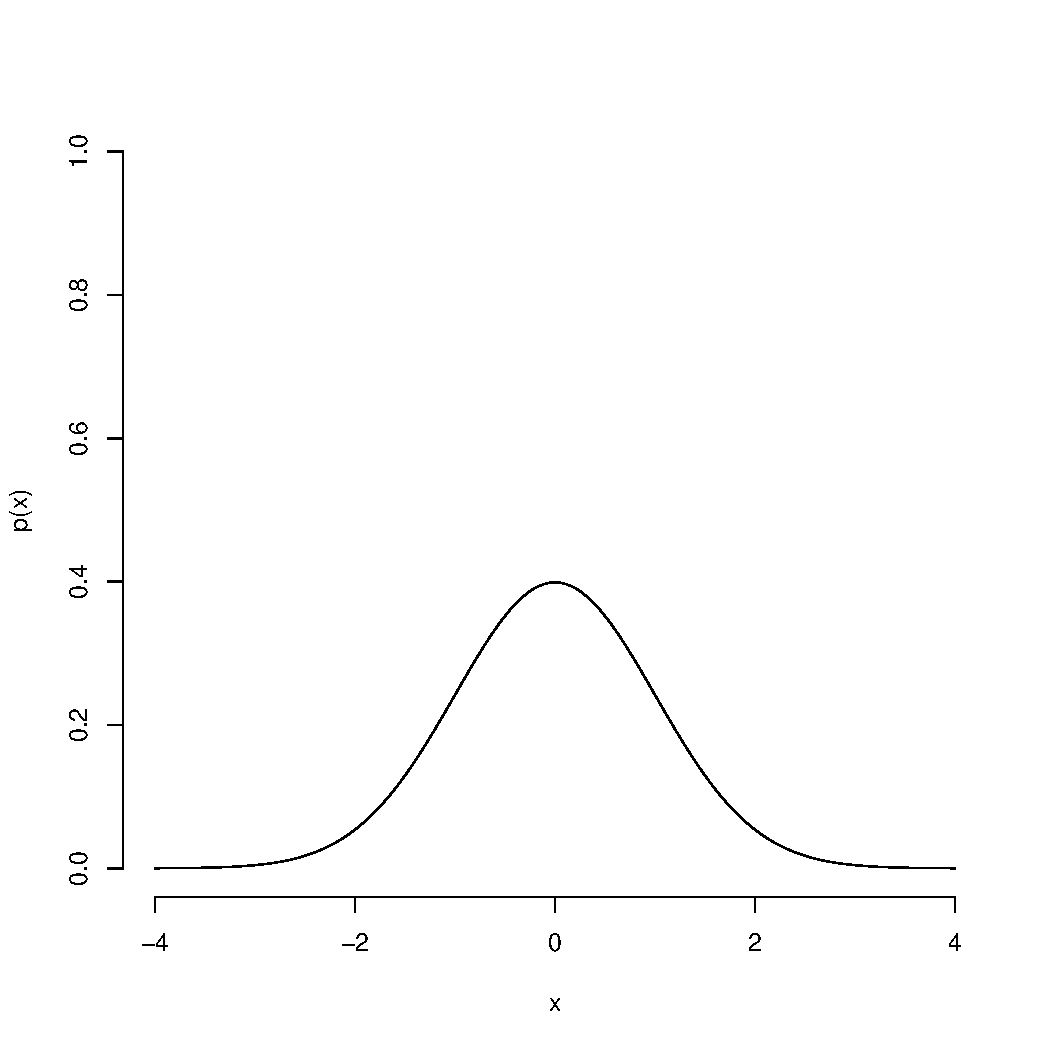
\includegraphics[width=.70\textwidth]{../distributions/normal/normal_bw.pdf}
\end{figure}
\marginnote[-3.0in]{
    \begin{align*}
        & X \sim \text{Normal} (\mu, \sigma^2) \\
        & -\infty < x < \infty \\
        & -\infty < \mu < \infty \\
        & 0 < \sigma^2 < \infty \\
        & p(x) = \frac{1}{\sqrt{2\pi\sigma^2}}\exp\left[-\frac{(x
            -\mu)^2}{2\sigma^2} \right] \\
        & \mu = E[X] = \mu \\
        & \sigma^2 = E[(x-\mu)^2] = \sigma^2 \\
    \end{align*}
}

\end{document}
